\documentclass[a4paper]{article}

%%
%% Packages in use.
%%
\usepackage[english]{babel}
\usepackage{hyperref}
\usepackage{listings}
\usepackage[T1]{fontenc}
\usepackage{avant}
\usepackage{color}
% The following is needed in order to make the code compatible
% with both latex/dvips and pdflatex.
\ifx\pdftexversion\undefined
\usepackage[dvips]{graphicx}
\else
\usepackage[pdftex]{graphicx}
\DeclareGraphicsRule{*}{mps}{*}{}
\fi

%%
%% Configuration of the document properties.
%%
\definecolor{codebackground}{rgb}{0.9,0.9,0.9}
\lstset{language=Java, basicstyle=\footnotesize, numbers=left, numberstyle=\tiny, escapeinside={//*}{\^^M}, frame=none, fontadjust=true, backgroundcolor=\color{codebackground}}
\usepackage{fullpage}
\addtolength{\oddsidemargin}{0.3cm}
\addtolength{\evensidemargin}{0.3cm}
% No indentation at start of a paragraph.
%\setlength{\parindent}{0in}
\renewcommand*\familydefault{\sfdefault}

%% 
%% Title information
%%
\title{Introduction to Hessian4J}
\author{Roger Laenen \and Bruno Ranschaert}

\begin{document}
\maketitle
\tableofcontents

%%
%% SECTION - WHAT IS HESSIAN
%%
\section{What is Hessian?}

In a nutshell, Hessian is a binary data transfer protocol with the following characteristics :

\begin{itemize}
	\item It is completely self describing, class definitions are contained within the data stream. The stream is self contained, no separate definition files are needed. 
	\item It is language agnostic, various language implementations currently exist. 
	\item It is compact in comparison with the hyped XML stuff. XML was invented to annotate documents whereas Hessian was invented to represent binary data in a standard way.
	\item It's a stateless protocol.
\end{itemize}

All grants for the protocol go to Caucho\footnote{\url{http://www.caucho.com/resin-3.0/protocols/hessian.xtp}} who defined the protocol and submitted it in 2007 as an IETF\footnote{\url{http://www.ietf.org}} draft. This article doesn't cover the internals of the protocol, more information on this can be found on the Caucho website itself.

The Java implementation discussed in this document, named Hessian4J, differs from the Caucho implementation in 2 ways :

\begin{itemize}
	\item It only supports the more recent (and more compact) version 2 of the protocol.
	\item The transformation from Java objects to the Hessian wire data is performed through an intermediate model. 
\end{itemize}

This last item was our primary motivation to create an alternative implementation. The existance of an intermediate Hessian model permits processing of the data (transformation, validation, routing,...) without requiring the existance of the associated Java business model. If you are creating a web interface for example, all classes used in the definition of the interface have to be available on the client and on the server. An intermediate agent is now able to read and parse the Hessian stream without having to reconstruct the business model. The intermediate model in our Hessian imlementation is what the DOM model is for XML.

%%
%% SECTION WHAT IS IT GOOD FOR?
%%
\section{What's it good for?}

Hessian is a replacement for XML when you need something fast and simple while direct access to the data (using a text editor) is less important. It is fast because it was designed that way, the Hessian format allows very fast parsers. It is simpler then XML, compact and complete implementations can be found for many languages. 

Basically you can use it to stream any data to a file or over the network. Because Hessian is a very compact protocol most benefit will be gained in high load environments. In a RESTful\footnote{Representational state transfer (REST) is a style of software architecture for distributed hypermedia systems such as the World Wide Web. See \url{http://en.wikipedia.org/wiki/Representational_State_Transfer}} environment you could use Hessian as the payload of your HTTP-POST request. Specifically for this purpose there is a separate draft proposal submitted to the IETF by Caucho. Examples where Hessian can be used:

\begin{itemize}
   \item Persist data to a file. 
   \item Use it to call a network service.
   \item Use it to post messages on an ESB.
\end{itemize}

%%
%% SECTION - BASIC CONCEPTS
%%
\section{Basic concepts}

\smallskip
\begin{figure}[htp]
\centering
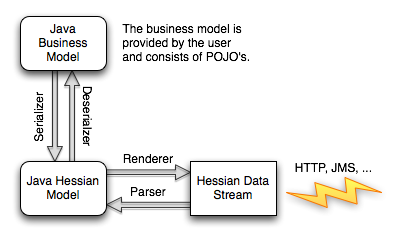
\includegraphics[scale=0.8]{concept.png}
\caption{2-phase transformation}
\label{fig:concept}
\end{figure}
\smallskip

As mentioned before the Hessian4J implementation transforms your Java model to the Hessian format through an intermediate model. This is illustrated in Figure \ref{fig:concept}.

Translating this to the software architecture we get the following :

\begin{itemize}
	\item \emph{HessianSerializer} class which does the serializing and deserializing. The terms "serialize" and "deserialize" mean the conversion between your Java object model and the Hessian object model.
	\item \emph{HessianParser} class which parses the Hessian data stream to the Hessian model. The term "parse" means to read something in Hessian and convert it to the Hessian object model.
	\item The Hessian model classes that are able to render themselves to the Hessian wire data format. The term "render" means to write a Hessian object representation to a Hessian encoded stream.
\end{itemize}

The Hessian model in fact is a hierarchical Java representation of the Hessian data types. The following figure illustrates its  basic structure :

\smallskip
\begin{figure}[htp]
\centering
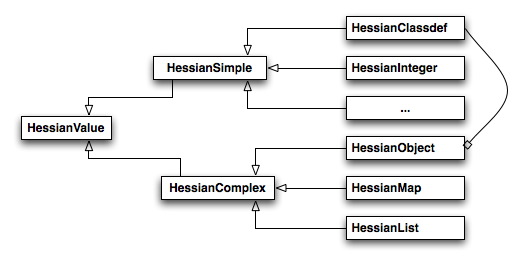
\includegraphics[scale=0.8]{model.png}
\caption{Structure of the Hessian model}\label{fig:model}
\end{figure}
\smallskip

%%
%% SECTION - SERIALIZATION
%%
\section{The serialization phase}

Let's first discuss the serialization from a Java object to its Hessian model representation. This process is driven by the \emph{HessianSerializer}. The serializer performs its task with the assistance of a set of hierachically structured \emph{helpers}. A so-called helper knows how to (de)serialize a specific class to/from the Hessian model. The HessianSerializer contains a repository with a predefined set of helper classes. You can add your own helper class to this repository if needed. It is the responsibility of these helpers to convert your Java objects to a corresponding Hessian model and vice-versa. Let's look at the following example :

\medskip
\begin{lstlisting}
HessianSerializer lSer = new HessianSerializer(); //* \label{createserializer} 
HessianValue lVal = lSer.serialize(myObject); //* \label{serializeobject}
\end{lstlisting}
\medskip

That's all there is. On line \ref{createserializer} a serializer is created. On line \ref{serializeobject} your java object is transformed to a Hessian representation and is ready to be rendered to a stream.

\subsection{What's a \emph{helper} ?}

Like we said before, you can add your own helper to the serializer repository. 
One of the most common cases you will need to do this is when you are dealing with Java classes that have no default constructor.
Normally, the deserializer will instantiate the Java object using reflection to call the default constructor.
For classes without a default constructor you have to write a Helper class that tells the serializer how to serialize and deserialize objects of it. Another common use of Helpers is where you want to transform your object (eg limit the number of attributes, convert a type..) before putting it on the wire. To give you an idea of the use of these helpers, take the following snippet:

\medskip
\begin{lstlisting}
final HessianSerializer lSerializer = new HessianSerializer();
lSerializer.getRepo().addHelper(new BigDecimalHelper());
HessianValue lVal = lSerializer.serialize(new BigDecimal("10.00"));
System.out.println(lVal.prettyPrint()); //* \label{prettyprint}
BigDecimal lResult = (BigDecimal) lSerializer.deserialize(lVal);
\end{lstlisting}
\medskip

As you notice on line \ref{prettyprint}, you can always prettyPrint a HessianValue to inspect the Hessian representation. We (de)serialize a BigDecimal here. BigDecimal is one of those classes without a default constructor, that's where our BigDecimalHelper\footnote{This helper is defined by default in the repository.} comes in.  What the helper basically does is converting our Java BigDecimal representation to a HessianObject with a HessianString argument. The value of this argument is the toString() value of the original BigDecimal. When consequently deserializing, the same helper will call the BigDecimal(String) constructor with the value of the string argument. Basically, the real (de)serialization work is done within the Helper classes, the HessianSerializer mainly keeps the context (more on this later).

When writing your own helper, there is a generic GenObjectHelper class you can extend from or you can make your own from scratch by implementing the HessianHelper interface.  When (de)serializing Java objects that don't have a specific Helper class we fall back to one of the 2 generic object helpers, ObjectHelper or ObjectHelperDirect. The difference between the 2 is the approach they take to read/write the attributes. ObjectHelper uses the JavaBean approach and as such calls the getters/setters of the object.  The ObjectHelperDirect implementation on the contrary uses reflection to directly access your attributes. By calling the setFieldAccess() method on the HessianSerializer you can switch between these 2. 
By default, direct field access is used.

\subsection{What's a ``namer''?}

Besides the Helpers another facility that is used by the (de)serializer is the Namer. The Namer translates between Java class names and corresponding Hessian names and vice-versa. This can be useful if the consumer of your data uses another naming convention or uses another programming languaga alltogether. The type names and class names in the Hessian model do not have to correspond to Java class names. The namers allow you to replace the automatically generated Java names with your own names. Namers are chained, when serializing each class-name encountered is passed to the namer chain.

The following example illustrates this :

\medskip
\begin{lstlisting}
public class NamerSample
{
    public static class BigDecimalNamer 
    implements Namer
     {
        public String mapHessian2Java(String aHessianName) 
        throws HessianSerializerException
        {
            if ("FOO".equals(aHessianName))
                return "java.math.BigDecimal";
            return aHessianName;
        }

        public String mapJava2Hessian(String aJavaName) 
        throws HessianSerializerException
        {
            if ("java.math.BigDecimal".equals(aJavaName))
                return "FOO";
            return aJavaName;
        }
    }

    public static void main(String[] args) 
    throws HessianSerializerException
    {
        final HessianSerializer lSerializer = new HessianSerializer();
        lSerializer.addNamer(new BigDecimalNamer());
        HessianValue lVal = lSerializer.serialize(new BigDecimal("10"));
        System.out.println(lVal.prettyPrint());

        BigDecimal bd = (BigDecimal)lSerializer.deserialize(lVal);
    }
}
\end{lstlisting}
\medskip

In this sample we serialize a BigDecimal as class FOO and deserialize it again to a BigDecimal.  One example of the use of namers is the \lstinline$WipeHibernateNamer$. When working with Hibernate you don't always want to transfer the Hibernate specific collection classes to your client app. In that case, you can add the WipeHibernateNamer which will translate the respective collection names to their Java equivalents. 

\subsection{Annotations}

When talking about helpers we mentioned the usage for classes without a default constructor. However, when you have full control over the class there is a simpler way to come around this problem. Hessian4J provides 2 annotations for this purpose, namely \lstinline$@HessianConstruct$ and \lstinline$@HessianSerialize$.


The method annoted with HessianSerialize should return an array of objects that can be passed (in the given order) to the constructor annotated with the HessianConstruct annotation. Using this approach avoids having to write a Helper class. 
The following snippet illustrates this :

\medskip
\begin{lstlisting}
public static class MyDate
{
    private Date theDate;
    private String theTimeZone;

    @HessianConstruct
    public MyDate(long aTime, String aTimeZone)
    {
        theDate = new Date(aTime);
        theTimeZone = aTimeZone;
    }

    @HessianSerialize
    public Object[] getTime()
    {
        return new Object[] {theDate.getTime(), theTimeZone};
    }
}
\end{lstlisting}
\medskip
    
%%
%% SECTION - RENDERER
%%
\section{The renderer}

There is no real Hessian renderer, instead each Hessian model class is able to render itself to the Hessian wire protocol format by calling its
render() method. The result of the rendering is put in the OutputStream you pass to it.
If you want to play a bit around with it, then just pass it a FileOutputStream and use your favorite HEX-editor to view the Hessian data.

Besides the OutputStream the render method expects another 3 list-arguments, 'types', 'classdefs' and 'objects'. A renderer uses these to make references to classes or objects that have already been rendered in the same context. The types list is used for to store the type of maps or lists (eg ArrayList, LinkedList...) in order to be able to reference it once the same collection type occurs more then once in the data stream.

%%
%% SECTION - PARSER
%%
\section{The parser}

The HessianParser sequentially reads and parses the given Hessian input stream to transform it into a HessianValue. It's a one-pass parser which makes the parsing very fast.  Note that the parser is not thread-safe (parsing information is stored internally), so every parsing thread should instantiate its own parser.

The use of the parser is very straightforward, instantiate it giving it an inputstream and call the nextValue() method to parse the first available data element in the stream. 

\medskip
\begin{lstlisting}
HessianParser lMyParser = new HessianParser(new FileInputStream(tempFile));
final HessianValue lMyString = lMyParser.nextValue();
\end{lstlisting}
\medskip

%%
%% SECTION - DESERIALIZER
%%
\section{The deserializer}

The deserialization takes the same approach as the serialization, it uses the same mechanism of namers and helpers to convert your Hessian value to the corresponding Java object.

Just invoke it by calling the deserialize() method passing it your HessianValue like in the following example :

\medskip
\begin{lstlisting}
Order lOrder2 = (Order) serializer.deserialize(aHessianValue);
\end{lstlisting}
\medskip

%%
%% SECTION - EXAMPLE
%%
\section{A simple example showing it all}

To summarize this quickstart, consider the following snippet, which serializes and renders an order to a ByteArrayOutputStream and subsequently parses and deserializes it again to its Java representation.

\medskip
\begin{lstlisting}
public class OrderSample
{
    public static class Order
    {
        private Date orderDate = new Date();
        private BigDecimal totalAmt = BigDecimal.ZERO;
        private Set<OrderLine> orderLines = new HashSet();

        public void addOrderLine(OrderLine aLine)
        {
            orderLines.add(aLine);
            totalAmt = totalAmt.add(
                aLine.unitAmount.multiply(
                    new BigDecimal(aLine.quantity)));
        }
    }

    public static class OrderLine
    {
        private String description;
        private int quantity;
        private BigDecimal unitAmount;

        public OrderLine() {}
        
        OrderLine(String aDescription, int aQuantity, BigDecimal anAmount)
        {
            description = aDescription;
            quantity = aQuantity;
            unitAmount = anAmount;
        }
    }

    public static void main(String[] args) 
    throws HessianSerializerException, 
                 HessianRenderException, 
                 HessianParserException
    {
        Order lOrder = new Order();
        lOrder.addOrderLine(new OrderLine("firstLine",1,new BigDecimal("10")));
        lOrder.addOrderLine(new OrderLine("secondLine",5,new BigDecimal("5")));

        HessianSerializer serializer = new HessianSerializer();
        HessianObject lVal = (HessianObject)serializer.serialize(lOrder);

        final ByteArrayOutputStream lOut = new ByteArrayOutputStream();
        lVal.render(lOut);
        System.out.println(lVal.prettyPrint());

        HessianParser lParser = new HessianParser(
            new ByteArrayInputStream(lOut.toByteArray()));
        HessianValue lVal2 = lParser.nextValue();

        Order lOrder2 = (Order) serializer.deserialize(lVal2);
    }
}
\end{lstlisting}
\medskip

%%
%% SECTION - NEXT
%%
\section{What next ?}

This concludes this quick guide to Hessian4J. In another issue we will cover the Hessian webservice specification which defines the use of Hessian in a webservice context.  The current implementation provides already the basic elements as defined in the draft\footnote{\url{http://hessian.caucho.com/doc/hessian-ws.html}}. Please download the software (its licensed as LGPL\footnote{GNU Lesser General Public License. See more at \url{http://www.gnu.org/licenses/lgpl.html}. In short, you can use it for commercial and non-commercial purposes, as long as you distribute the license text of Hessian4J as well.}) and try it out. All feedback, positive or negative, is welcome.  Currently we're working on integration with the Spring framework for a next release.

\end{document}
